\section{Блокчейн Asure}
С технической точки зрения системы социального обеспечения можно охарактеризовать как ряд основанных на правилах (финансовых) операций, которые осуществляются между (обычно) незначительно изменяющейся совокупностью различных сторон при условии поддержания равновесия между депонированной и выведенной стоимостью в течение определенного периода времени. Такая система может быть реализована в цифровом виде путем создания блокчейн-системы, которая поддерживает смарт контракты и криптовалюты.

Обычные системы социального обеспечения в настоящее время генерируют до сотен миллионов транзакций в месяц, это зависит от количества участвующих сторон и конкретного варианта использования социального обеспечения. 

\begin{table}[H]
\centering
\begin{tabular}{lp{.2\textwidth}l}
  Ежемесячные пенсионные взносы & = 54.445 Mio\\
  Ежемесячные пенсии & = 25.646 Mio\\\hline
  Ежемесячные пенсионные операции & = 80.091 Mio
\end{tabular}
\caption{\label{tab:table-name} Например, немецкая система пенсионного обеспечения: \cite{eckzahlen}}
\end{table}

Чтобы разработать систему блокчейн, которая сможет обрабатывать все эти транзакции, необходимо увеличить достижимую пропускную способность транзакций системы и автоматическую пакетную обработку внутри транзакции, чтобы уменьшить общее количество транзакций до минимума.

Оба требования могут быть решены путем использования сайдчейна, как указано в Plasma Framework. Блокчейн Asure функционирует как масштабируемый сайдчейн реализации Asure Plasma. Это рутчейн сети Asure и закладывает основу для оптимальной масштабируемости в отношении систем социального обеспечения на основе блокчейна. 

Активы, переданные из блокчейна Ethereum в один из сайдчейнов Asure, блокируются в контракте Asure Plasma на блокчейне Ethereum до тех пор, пока не будет выполнена транзакция выхода из блокчейна Ethereum. В соответствии со спецификациями Plasma MVP, эквивалент этого значения создается с помощью шаблона проектирования оператора (Proof-Of-Authority) в блокчейне Asure и присваивается пользователю.

Затем доступные активы в блокчейне Asure можно использовать для транзакций в системе. Консенсус между всеми провайдерами узлов в блокчейне Asure достигается с помощью алгоритма proof-of-stake с использованием адаптированной версии механизма консенсуса Tendermint. \cite{tendermint} Tendermint может обрабатывать объем транзакций до 10000 транзакций в секунду. С помощью зон и концепций шардинга этот размер можно увеличить в 1000 раз. Это обеспечит устойчивую работу системы социального обеспечения на блокчейне. \cite{tendermint_bench}

\begin{figure}[H]
    \centering
    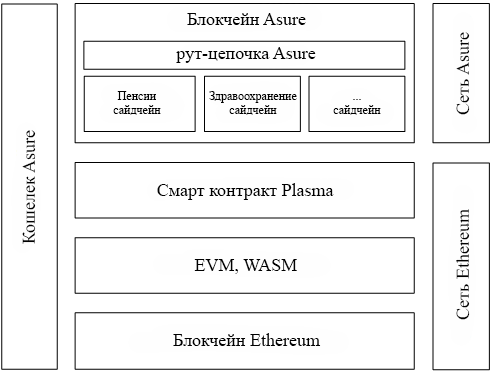
\includegraphics[width=4.0in]{img/architecture.png}
    \caption{Архитектура Asure}
    \label{fig:asure_architecture}
\end{figure}

У блокчейна Asure есть несколько основных принципов. 

\subsection{Безопасность}
Блокчейн Asure включает в себя несколько функций, которые защищают его от таких атак, как несанкционированные расходы, двойные расходы, подделка активов и вмешательство в блокчейн. 

Каждый блок, добавленный в блокчейн, начиная с блока, содержащего конкретную транзакцию, является подтверждением этой транзакции. В идеале получатели и отправители, получающие платежи, должны дождаться, пока хотя бы одно подтверждение не будет распространено по сети, прежде чем предполагать, что платеж был сделан. Чем больше подтверждений ожидает получатель, тем сложнее злоумышленнику успешно отменить транзакцию в блокчейне, если только злоумышленник не контролирует более половины всей производительности сети, то в этом случае это называется атакой на 51 процент. Эта платформа не предназначена для предотвращения таких атак, а скорее для поощрения распространения блоков. 

\subsection{Алгоритм Консенсуса}
Существуют разные версии алгоритмов доказательства. Proof-of-work подвергается резкой критике из-за огромного энергопотребления.\cite{hackernoon} Долгосрочное принятие и движение сообщества движутся к алгоритму proof-of-stake, где валидаторы создают блоки и получают вознаграждение за правильную работу. Блокчейн Asure будет использовать согласованный алгоритм Proof-of-Stake (PoS). В первой реализации MVP будет использоваться механизм консенсуса Tendermint.\cite{tendermint}

\subsection{Конфиденциальность с (ZK-SNARKS и ZK-STARK)}
Среди прочего, блокчейн Asure учитывает аспекты конфиденциальности, которые имеют огромное значение для социального обеспечения.

ZK-SNARKS (Zero-Knowledge Succinct Non-interactive Argument of Knowledge) дает возможность проводить анонимные транзакции. ZK-SNARKS не устойчивы к квантовым вычислениям. ZK-STARK (Zero-Knowledge Scalable Transparent Argument of Knowledge) это последнее новшество которое устойчиво к квантовым вычислениям и нацелено на достижение конфиденциальности в блокчейне с использованием быстрых масштабируемых вычислений. \cite{iacr}

Поскольку Ethereum также проводит исследования на уровне 1 в этой области, транзакции социального обеспечения могут оставаться анонимными для застрахованных пользователей. \cite{ethereum_zksnarks}

Использование технологии с нулевым разглашением еще не вполне осуществимо, но это изменится в будущем.

\subsection{EVM, WASM, eWASM, *WASM}
EVM обеспечивает тьюринг-полноту, так что Ethereum может запустить обычную программу, также известную как смарт контракт. Plasma EVM это новая версия Plasma, которая может выполнять EVM в ее цепочке и ее клиенты могут основываться на текущих клиентах Ethereum (go-ethereum, py-evm, parity). Мы предлагаем реализацию Plasma с принудительной проверкой состояния, чтобы гарантировать только правильное состояние, отправленное в рутчейн, предоставляя способ входа и выхода из хранилища учетных записей между двумя цепочками, поскольку каждая цепочка имеет идентичную архитектуру. Еще одним преимуществом является то, что инструменты разработки Ethereum также могут быть использованы в цепи Plasma.

eWASM это просто «приправленное» подмножество Ethereum WebAssembly, представляющее собой двоичный формат инструкций. eWASM опирается на инструкции, которые очень близки к реальному процессору. Улучшения производительности значительны и кажутся более безопасными. WebAssembly поддерживается Mozilla, Google, Apple и Microsoft, сообщество также активно, это будет широко используемый веб-стандарт. 

Блокчейн Ethereum обрабатывает около 15 транзакций в секунду (TPS), что недостаточно для внедрения системы социального обеспечения. Улучшения Ethereum (также называемые Layer 1), которые в настоящее время находятся в стадии разработки, должны значительно увеличить количество TPS. Улучшения включают в себя алгоритм консенсуса на основе Proof-of-Stake (PoS), шардинг, а также введение eWASM - виртуальной машины на основе WebAssembly.

\subsection{Другие технологии}
Parity Substrate это высокоуровневая структура для создания криптовалют и других децентрализованных систем с использованием новейших исследований в технологии блокчейн. 

Cosmos-SDK - это блокчейн платформа, позволяющая разработчикам легко создавать настраиваемые взаимодействующие блокчейн приложения в сети Cosmos Network без необходимости воссоздания общей функциональности блокчейна, что устраняет сложность создания приложения Tendermint ABCI. Мы рассматриваем SDK как npm-подобную инфраструктуру для создания защищенных блокчейн приложений поверх Tendermint.

LotionJS стремится сделать написание новых блокчейнов более быстрыми. Он построен поверх Tendermint с использованием протокола ABCI. Lotion позволяет создавать безопасные, масштабируемые приложения, которые могут легко взаимодействовать с другими блокчейнами в Cosmos Network.

